% =====================================================================
% overleaf/99_annexes.tex — LaTeX rendering of en/99_annexes.md draft v0 (17 September 2026)
% Dernière mise à jour : 2026-09-21
% Technical appendices of the paper. To be inserted AFTER \bibliography, at the very end of the document,
%   preceded in the main file by \appendix (this file does NOT issue \appendix itself, so that the main file
%   keeps control of where the appendix block starts).
% LABELS DEFINED HERE, all three referenced from earlier chapters and resolving to ?? until this file existed:
%   app:variables — Appendix E, the 21 variables. Referenced by overleaf/chapters/04_Evaluation.tex.
%   app:margins   — ATTACHED TO APPENDIX G, which is the nearest holder: chapter 4 references it for the
%                   microdata recomputations of the margins the published report does not carry, and NO appendix
%                   carries that margin-by-margin table today. Move the label if such an appendix is written.
%   app:detail    — Appendix H, the detailed results. Referenced by overleaf/chapters/06_Empirical_Evaluation.tex.
%   app:unit      — Appendix I, the unit audit. Referenced by overleaf/chapters/06_Empirical_Evaluation.tex.
% TWO THINGS TO TAKE UP IN APPENDICES A TO G before submission, inherited from the French draft and NOT
%   repaired by the rendering: the figures, to be cross-checked from the repository rather than copied from
%   here; the cross-references, which followed the old manuscript numbering (rewritten as \ref here, still
%   hard-numbered in the Markdown master). Appendix H carries none of these.
% The "Tier 1 / 2 / 3" vocabulary left these appendices before 21 September 2026 — checked that day, not one
%   occurrence remains in fr/99, en/99 or this file's body. Should it ever come back, WITHDRAW it: Sections 1
%   and 2 reserve exploratory / robust / transferable for SILICA's certification steps, never for our own
%   conditions, so it cannot be renamed into them.
% Preamble additions:
%   \newcommand{\todo}[1]{\textbf{[#1]}}
% Figures: four, all PNG, all composed IN ENGLISH by scripts/analysis/plot_chapitre6.py, regenerated 2026-09-17.
%   The two figures of the unit audit are carried by overleaf/chapters/06_Empirical_Evaluation.tex, not by this file.
%   Caption BELOW, mandatory \Description. All four are set as figure* across both columns: they are multi-panel
%   plates and a single column makes them unreadable.
%   FILES TO UPLOAD to the Overleaf project, flat, next to the .tex:
%   ch99_dimensions_voiture.png, ch99_modes_distance.png, ch99_modes_occupation.png, ch99_modes_motif.png
%   (sources in docs/paper/article/images/).
% Tables: twelve, caption ABOVE, booktabs. The wide ones (variables, corrections, paired differences, error by
%   dimension, modal shares, agreement) are table* across both columns.
% Numbers: the Markdown decimal comma becomes a decimal point, the thousands separator a comma.
% Traceability: the "source:" comments live in the ../fr/ and ../en/ masters only. Do not carry them
%   over into this file when rendering a chapter into LaTeX (author's decision, 2026-09-21).
% Derived file: regenerate after every validated pass of en/99_annexes.md.
% =====================================================================


\section{API quota summary and the Antigravity platform}
\label{app:quotas}

Inference rests on the SWRR API gateway (\texttt{llm\_module}, 11 instances, 206 RPM / 37{,}700+ RPD) and on the Google Antigravity agentic environment (Gemini 3.6 Flash and 3.5 Flash Lite, 1M token context, isolated sub-agents).

\section{Survey evaluation script}
\label{app:evalscript}

Blind inference script (\texttt{eval\_llm\_on\_survey.py}) over the 13{,}045 sealed trips of the EMC\textsuperscript{2} 2023 survey.

\section{Local inference configuration}
\label{app:qwen}

vLLM server \texttt{Qwen/Qwen2.5-32B-Instruct-AWQ} at $\tau = 0.0$ with a fixed seed.

\section{Calibration assessment and justification of the pivot}
\label{app:pivot}

Non-convex loss landscape justifying the pivot towards the hybrid architecture.

\section{Dictionary of the 21 variables of the comparison protocol}
\label{app:variables}

The comparison protocol of Section~\ref{sec:contract} designates the 21 variables of Table~\ref{tab:variables}, and them alone. The list is fixed in the repository (\texttt{spec\_version 2}) and it is that same file that builds the design matrix of the four tabular methods: neither the logit, nor gradient boosting, nor the random forest, nor the kernel regression sees anything else.

\begin{table*}[tp]
  \caption{The 21 variables of the comparison protocol, in three blocks. Every decider of Section~\ref{sec:levels} receives these, and the tabular references receive nothing else.}
  \label{tab:variables}
  \begin{tabular}{llp{0.52\textwidth}}
    \toprule
    Variable & Type & What it says \\
    \midrule
    \multicolumn{3}{l}{\textit{Person and household --- 12 variables}} \\
    \texttt{age}                      & numeric     & age in completed years \\
    \texttt{gender}                   & categorical & woman / man \\
    \texttt{household\_size}          & numeric     & number of people in the household \\
    \texttt{has\_driving\_license}    & boolean     & the person holds a driving licence \\
    \texttt{has\_pt\_subscription}    & boolean     & the person has a public transport pass \\
    \texttt{number\_of\_cars}         & numeric     & cars of the household \\
    \texttt{car\_availability}        & categorical & car available to all adults, to some, to none \\
    \texttt{has\_bike}                & boolean     & the person has a bicycle \\
    \texttt{socioprofessional\_class} & categorical & socio-professional category, 8 modalities \\
    \texttt{main\_occupation}         & categorical & main occupation, 8 modalities \\
    \texttt{employed}                 & boolean     & the person holds a job \\
    \texttt{studies}                  & boolean     & the person is in education \\
    \midrule
    \multicolumn{3}{l}{\textit{Trip context --- 3 variables}} \\
    \texttt{purpose}                  & categorical & purpose of the destination activity: home, work, education, shopping, leisure, other \\
    \texttt{purpose\_origin}          & categorical & purpose of the origin activity, same modalities \\
    \texttt{departure\_hour}          & numeric     & departure time, in decimal hours \\
    \midrule
    \multicolumn{3}{l}{\textit{Geography --- 6 variables}} \\
    \texttt{od\_km}                   & numeric     & straight-line origin--destination distance \\
    \texttt{same\_zone}               & boolean     & origin and destination in the same fine zone of the survey \\
    \texttt{dist\_center\_orig\_km}   & numeric     & distance from the origin to the inner centre \\
    \texttt{dist\_center\_dest\_km}   & numeric     & distance from the destination to the inner centre \\
    \texttt{density\_orig}            & numeric     & population density of the origin zone \\
    \texttt{density\_dest}            & numeric     & population density of the destination zone \\
    \bottomrule
  \end{tabular}
\end{table*}

The inner centre is the centroid of the fine zones of the Capitole sector, and the distances are computed in the legal projection. A 19-variable variant, without the two distances to the inner centre, has been measured, accuracy \todo{xx} and composite \todo{xx}, and two alternative definitions of distance were set aside; the protocol served is the 21-variable one. What the agent receives in addition to these 21 variables, the agenda of its remaining trips, the weather of the coming time slots and the itineraries themselves, is described in Section~\ref{sec:contract}.

\section{Log of methodological corrections}
\label{app:corrections}

Every figure of the manuscript was cross-checked against the measurements the repository produces. Table~\ref{tab:corrections} lists the gaps corrected.

\begin{table*}[tp]
  \caption{Methodological corrections applied between versions 1.3 and 1.6 of the detailed manuscript. Cross-checking sources: \texttt{mode\_choice\_policy\_metrics.json}, \texttt{feature\_spec.json}, \texttt{docs/arch/score-synthesis.md}, \texttt{docs/changelog.md}.}
  \label{tab:corrections}
  \begin{tabular}{rp{0.42\textwidth}p{0.42\textwidth}}
    \toprule
    \# & Gap found & Correction applied \\
    \midrule
    1 & ``15 variables'' at informational parity & Production contract at 21 variables (\texttt{spec\_version 2}) \\
    2 & L1 of the tabular reference (2.68) set against that of the LLM (29.81) & Probability mass against argmax: comparison brought back to 7.30 against 29.81 \\
    3 & ``$\chi^2$, $p = 0.98$ confirms perfect fidelity'' & Non-rejection is not proof; replaced by an equivalence test and effect sizes \\
    4 & Milestone 0 presented as a validation & Requalified as a coherence check; cross-tabulations still to test \\
    5 & Composites compared with no sample size & Sample size now mandatory: $+5.02$ pt measured at constant decisions when going from 881 to 81 people \\
    6 & Parity presented as symmetric & Exposure asymmetry declared, 31{,}279 trips seen against zero, and a few-shot condition added \\
    7 & ``Tabular model blind to the event'' & It is not blind, it is not informed, hence condition C5, the tabular reference receiving the encoded event \\
    8 & Press effect measured against a condition with no article & Addition of the paraphrase with no modal cue and of the placebo article \\
    9 & ``$10{,}000\times$ faster'' & Withdrawn. The ratio announced next, about $2{,}700\times$, came from the comparative table of the manuscript and not from a measurement; no source was found. Set aside pending measurement \\
    10 & Perimeter of the unit audit, 1{,}000 against 13{,}045 trips & Perimeter unified: the nine deciders are measured on the same ground, 9{,}621 trips declared by 2{,}930 respondents, each on their own day and survey date. The tabular landmarks on 13{,}045 remain published in Section~\ref{sec:audit}; they hold outside the vehicle chain and are not commensurable \\
    11 & Composite weights announced at $0.40 / 0.20 / 0.20 / 0.20$ with $\sum w = 1$ & Weights actually served: global 1.0, absence 1.0, age 0.5, occupation 0.5, purpose 0.5, gender 0.3, distance 0.3; weighted sum, not renormalised \\
    12 & Demographic conformity table with no source, matching neither the published report nor the measured reference population & Targets replaced by those of the report and, for the unpublished margins, by frozen recomputations on microdata; cohort measured by \texttt{control\_population.py}, 13 margins, TOST $\pm 1$ pt \\
    \bottomrule
  \end{tabular}
\end{table*}

\section{Source of the survey data, citation and usage commitments}
\label{app:margins}

The tabular references of this paper are fitted on the microdata of the Cerema-certified household travel survey of the greater Toulouse area, EMC\textsuperscript{2} 2023, obtained from Quetelet-Progedo-Diffusion under agreement \texttt{lil-1750}. The citation template annexed to the agreement imposes the wording carried by the footnote of Section~\ref{sec:substrate}, to within one vintage: the template as delivered carries ``2013'' where the survey used in this work is that of 2023. The DOI remains the one the distributor assigned to the order. Bibliographic entries: \texttt{tisseo2023emc2} for the published report, \texttt{progedo2023emc2microdata} for the distributed file.

\paragraph{Obtaining the data.} The microdata are distributed to research through the Quetelet-Progedo-Diffusion portal (ADISP). The record to request is the \textit{Enqu\^ete Mobilit\'e Certifi\'ee Cerema (EMC\textsuperscript{2}) de la Grande Agglom\'eration Toulousaine, 2023}. The request is made online: account creation, selection of the survey in the catalogue, declaration of the research project, signature of the commitment recalled below. The agreement for this work carries its own number; a third party obtains theirs, under their own. No approach to the authors is necessary, and none replaces that one: the commitments forbid transfer.

\paragraph{What the agreement commits to.} Research use only; no transfer of the data to a third party, in any form whatsoever; processing in accordance with the state of the art and with statistical confidentiality; registration of the research in the institution's processing declaration register; compliance with personal data regulation; mention of the source in communications and publications; information of the distributor about communications, quality findings and any reuse; storage in an encrypted space during the research; destruction of the files at its end.

\paragraph{Replaying the fit.} The files received are placed as they are under \texttt{data/PROGEDO 2023/}: the three standard files and the fine-zone layer. \texttt{build\_mode\_choice\_dataset.py} then rebuilds the training set and its split, made by household (\texttt{GroupShuffleSplit} on the household identifier, 25\,\%, seed 0), so that the 13{,}045 test trips come back identically, with no household straddling the two sides. The four methods are then refitted by \texttt{fit\_mode\_choice\_\{policy,logit,klr,forest\}.py}, and the figures published in Section~\ref{sec:references} are recomputed from the \texttt{*\_metrics.json} files produced.

\paragraph{Consequence for the supplementary material.} The boundary runs there: the archive carries the code, the experiment configurations, the seeds and the sealed synthetic cohort with its demographic control manifest, everything that can be audited with no procedure. It carries neither the microdata, nor the sealed test set of 13{,}045 trips, nor any file that would reproduce its content. The itinerary offer submitted to the agents is not part of it either, for its size and not for its status: it regenerates from the cohort through the routing engines, and the manifest of the set seals the fingerprints that allow a check that the rebuilt set is the same one. A reviewer therefore checks the cohort, the protocol and the scores immediately, and the training side of the tabular references after a request to the distributor.

\paragraph{The same reading on drawn modes.} The runs of Section~\ref{sec:references}, read on the mode drawn from the mass rather than on the mass itself, give the composite EMD--JSD of Table~\ref{tab:drawn}. The gap with the reading by mass measures the noise of the draw, and it does not go the same way for all of them. The order of the four methods changes twice with respect to the mass: the random forest passes ahead of the logit it followed, and the kernel regression ahead of gradient boosting.

\begin{table}[tbp]
  \caption{The four tabular references read on the drawn mode. In brackets, the gap with the reading by probability mass.}
  \label{tab:drawn}
  \small
  \setlength{\tabcolsep}{4pt}
  \begin{tabularx}{\columnwidth}{@{}Lr@{}}
    \toprule
    Reference method & \multicolumn{1}{c}{Composite EMD--JSD,} \\
                     & \multicolumn{1}{c}{drawn modes} \\
    \midrule
    Gradient boosting (LightGBM)  & 3.88 ($+0.28$) \\
    Multinomial logit             & 4.54 ($+0.52$) \\
    Kernel logistic regression    & 3.52 ($-0.08$) \\
    Random forest                 & 4.40 ($+0.31$) \\
    \bottomrule
  \end{tabularx}
\end{table}

% FOR THE FINAL VERSION: the mention of the processing declaration register, which names the institution, does not
%   appear in the double-blind submitted version. Add it here for the non-anonymous version, with the
%   acknowledgements to the distributor.

\section{Detailed results}
\label{app:detail}

Section~\ref{sec:results} publishes only the lessons; this appendix carries the complete tables they rest on. Substrate: the sealed cohort, 3{,}154 scored decisions, 868 mobile people. Every decider is measured on it.

\subsection{The paired differences, on the three readings}

Cluster resampling at the person level, 2{,}000 replicates, seed 2026, 868 people common to both sides. In Table~\ref{tab:paired}, a positive gap is a higher error for the first term; in bold, the intervals that do not contain zero.

\begin{table*}[tp]
  \caption{The fourteen paired differences, on the three readings of the protocol. Bold marks an interval that excludes zero.}
  \label{tab:paired}
  \small
  \setlength{\tabcolsep}{4pt}
  \begin{tabular}{@{}lccc@{}}
    \toprule
    Paired difference & Composite & Excl.\ single choice & L1 global shares \\
    \midrule
    \texttt{gemini-3.5} expert $-$ minimal        & $\mathbf{-2.27}\ [-3.22; -1.40]$ & $\mathbf{-3.59}\ [-4.83; -2.45]$ & $\mathbf{-10.2}\ [-12.5; -8.0]$ \\
    \texttt{gemini-3.1} expert $-$ minimal        & $\mathbf{-3.37}\ [-4.25; -2.45]$ & $\mathbf{-4.15}\ [-5.22; -3.09]$ & $\mathbf{-8.6}\ [-10.6; -6.8]$ \\
    \texttt{mistral-large} expert $-$ minimal     & $\mathbf{-7.25}\ [-8.67; -5.90]$ & $\mathbf{-8.63}\ [-10.28; -7.15]$ & $\mathbf{-18.0}\ [-22.4; -13.5]$ \\
    \midrule
    \texttt{gemini-3.5} expert $-$ gradient boosting & $\mathbf{+1.35}\ [+0.28; +2.47]$ & $+1.09\ [-0.27; +2.45]$ & $+4.3\ [-1.2; +9.7]$ \\
    \texttt{gemini-3.5} expert $-$ kernel regression & $\mathbf{+1.38}\ [+0.32; +2.45]$ & $\mathbf{+1.35}\ [+0.10; +2.69]$ & $\mathbf{+7.1}\ [+1.8; +12.1]$ \\
    \texttt{gemini-3.5} expert $-$ random forest     & $+0.94\ [-0.06; +1.98]$ & $+1.17\ [-0.02; +2.39]$ & $\mathbf{+7.7}\ [+3.3; +11.7]$ \\
    \texttt{gemini-3.5} expert $-$ multinomial logit & $+0.96\ [-0.18; +2.17]$ & $+0.39\ [-1.10; +1.80]$ & $+4.4\ [-0.4; +8.5]$ \\
    \texttt{gemini-3.1} expert $-$ gradient boosting & $\mathbf{+5.50}\ [+4.19; +6.93]$ & $\mathbf{+6.65}\ [+5.21; +8.29]$ & $\mathbf{+21.7}\ [+16.6; +27.0]$ \\
    \texttt{mistral-large} expert $-$ gradient boosting & $\mathbf{+4.07}\ [+2.47; +5.75]$ & $\mathbf{+6.33}\ [+4.54; +8.09]$ & $\mathbf{+17.2}\ [+12.7; +21.6]$ \\
    \midrule
    \texttt{gemini-3.1} $-$ \texttt{gemini-3.5}, expert     & $\mathbf{+4.15}\ [+2.99; +5.43]$ & $\mathbf{+5.56}\ [+4.12; +7.02]$ & $\mathbf{+17.4}\ [+14.6; +20.3]$ \\
    \texttt{gemini-3.1} $-$ \texttt{gemini-3.5}, minimal    & $\mathbf{+5.25}\ [+4.11; +6.40]$ & $\mathbf{+6.13}\ [+4.75; +7.53]$ & $\mathbf{+15.8}\ [+13.2; +18.3]$ \\
    \texttt{mistral-large} $-$ \texttt{gemini-3.5}, expert  & $\mathbf{+2.71}\ [+1.17; +4.25]$ & $\mathbf{+5.24}\ [+3.76; +6.66]$ & $\mathbf{+12.8}\ [+8.3; +17.4]$ \\
    \texttt{gemini-3.1} $-$ \texttt{mistral-large}, expert  & $+1.44\ [-0.10; +2.98]$ & $+0.32\ [-1.14; +1.82]$ & $+4.6\ [-0.1; +9.0]$ \\
    \texttt{gemini-3.1} $-$ \texttt{mistral-large}, minimal & $\mathbf{-2.45}\ [-4.08; -0.85]$ & $\mathbf{-4.16}\ [-5.89; -2.45]$ & $\mathbf{-4.8}\ [-7.4; -2.2]$ \\
    \bottomrule
  \end{tabular}
\end{table*}

The ranking of the models changes with the instruction. Under the minimal prompt, \texttt{gemini-3.1} is ahead of \texttt{mistral-large} by 2.45 points, an interval excluding zero; under the expert prompt, \texttt{mistral-large} passes back ahead by 1.44, an interval containing zero. A benchmark run under a single instruction therefore measures the model--instruction couple, not the model.

The ablation of the justification clause, which asked the agent to explain why walking does not get the highest probability, is worth $+0.17$ $[-0.45; +0.79]$ point on its removal: taking it out improves the composite, without the interval excluding zero. It is measured on the earlier substrate, the variant that carried it having been removed from the repository.

\subsection{The error by dimension and by decider}

Table~\ref{tab:dimensions} gives the mean of the stratum L1 errors, weighted by the size of the covered strata. The dimensions entering the composite are age, gender, occupation, purpose and distance; the residential ring and the housing type enter neither the composite nor the calibration cycle.

\begin{table*}[tp]
  \caption{Weighted L1 error (\%) by dimension and by decider. In bold, the lowest error of each column: distance is the only dimension where an agent holds it.}
  \label{tab:dimensions}
  \begin{tabular}{lrrrrrrr}
    \toprule
    Decider & distance & purpose & age & occupation & gender & ring & housing \\
    \midrule
    \texttt{gemini-3.5}, minimal    & 24.1 & 27.9 & 30.6 & 25.3 & 23.9 & 25.7 & 30.5 \\
    \texttt{gemini-3.5}, expert     & \textbf{14.2} & 21.4 & 22.1 & 18.5 & 13.6 & 19.6 & 23.6 \\
    \texttt{gemini-3.1}, minimal    & 38.0 & 37.8 & 43.9 & 39.2 & 39.4 & 40.5 & 43.1 \\
    \texttt{gemini-3.1}, expert     & 30.2 & 30.8 & 35.8 & 31.2 & 30.7 & 33.0 & 37.4 \\
    \texttt{mistral-large}, minimal & 51.9 & 39.3 & 46.8 & 43.8 & 44.5 & 47.6 & 51.0 \\
    \texttt{mistral-large}, expert  & 33.7 & 27.9 & 30.4 & 28.6 & 25.3 & 29.6 & 33.0 \\
    \midrule
    Gradient boosting (LightGBM)    & 17.8 & \textbf{13.6} & 18.2 & 15.7 & 8.5 & 11.5 & 16.6 \\
    Random forest                   & 16.8 & 18.1 & \textbf{16.8} & \textbf{12.9} & \textbf{5.3} & \textbf{9.5} & \textbf{15.9} \\
    \bottomrule
  \end{tabular}
\end{table*}

\begin{figure*}[tp]
  \centering
  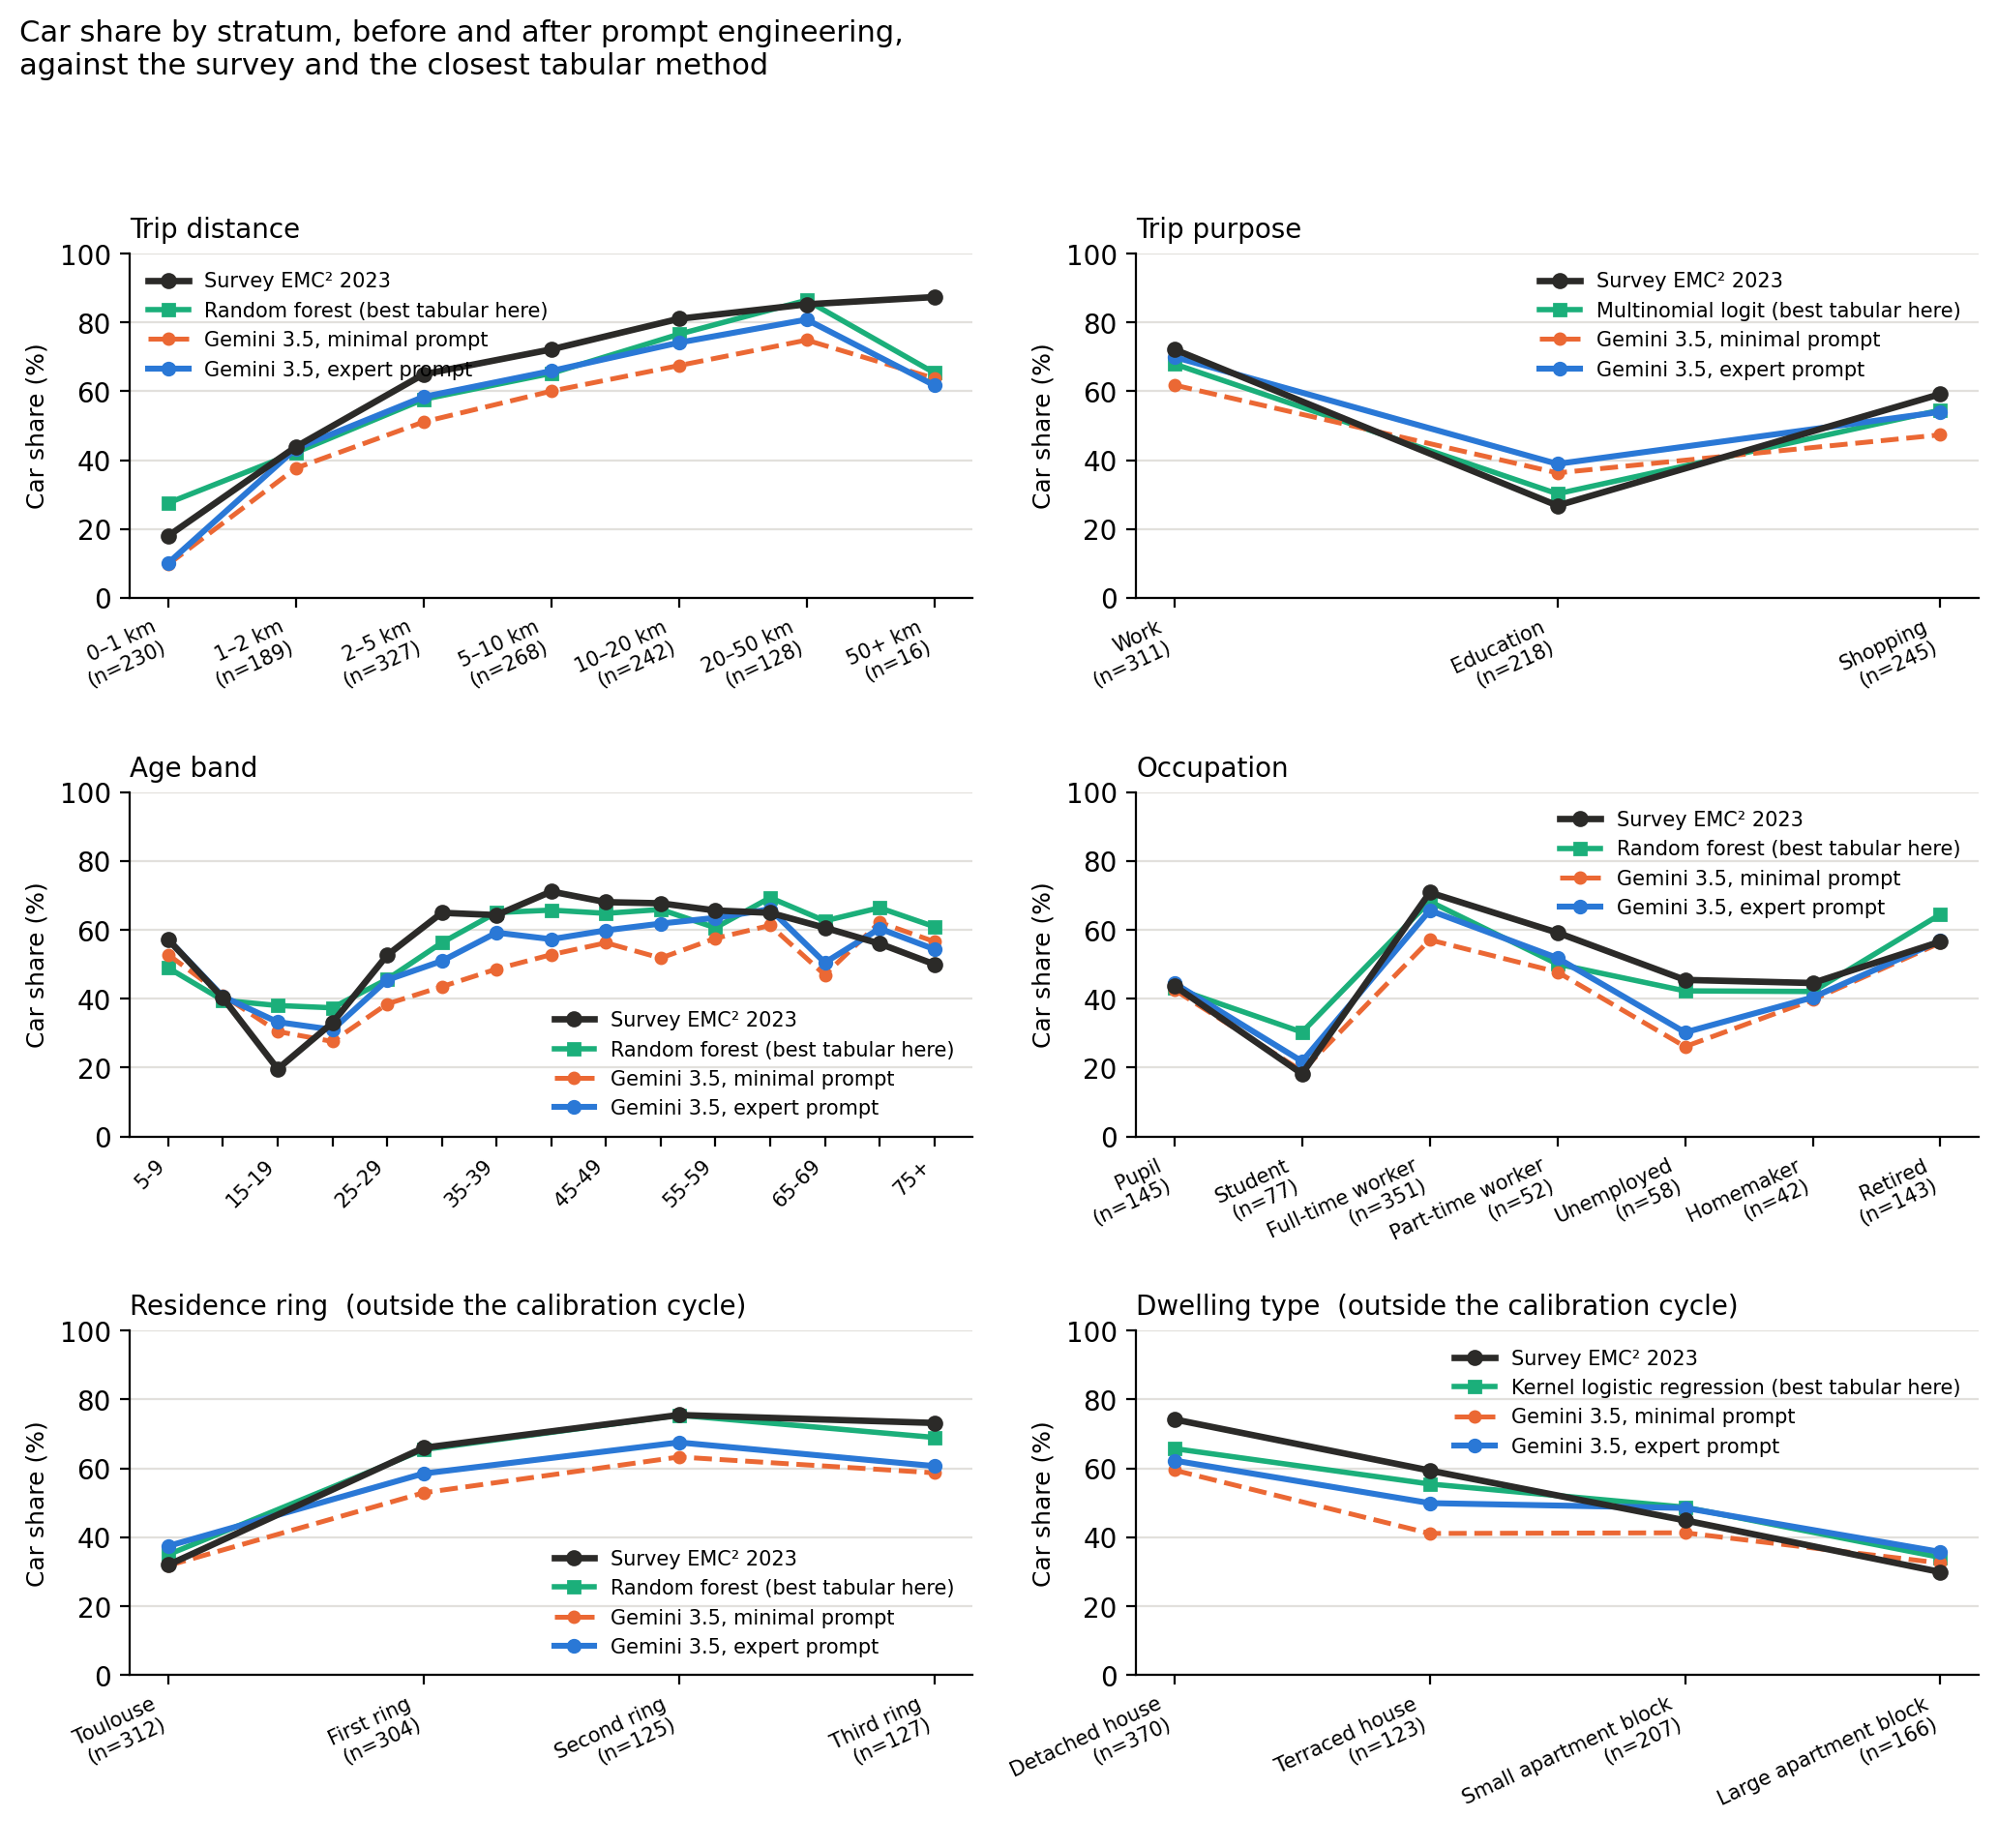
\includegraphics[width=\textwidth]{images/ch99_dimensions_voiture.png}
  \caption{The car share by stratum on six dimensions, before and after prompt engineering, against the survey target and the tabular method closest to that target on each dimension. The last two, residential ring and housing type, enter neither the composite nor the calibration cycle, and the gap stays wide there after tuning.}
  \label{fig:app-dimensions}
  \Description{Six panels, one per dimension: distance band, trip purpose, age band, occupation, residential ring and housing type. In each panel, the horizontal axis carries the strata of that dimension and the vertical axis the car share in per cent. Four series are plotted: the survey target, gemini-3.5 under the minimal prompt, the same model under the expert prompt, and the tabular method closest to the target on that dimension. On the first four panels the expert-prompt series sits closer to the target than the minimal-prompt series across most strata. On the last two panels, the residential ring and the housing type, the two agent series stay close to each other and both remain well away from the target, these dimensions entering neither the composite nor the calibration cycle.}
\end{figure*}

\begin{figure*}[tp]
  \centering
  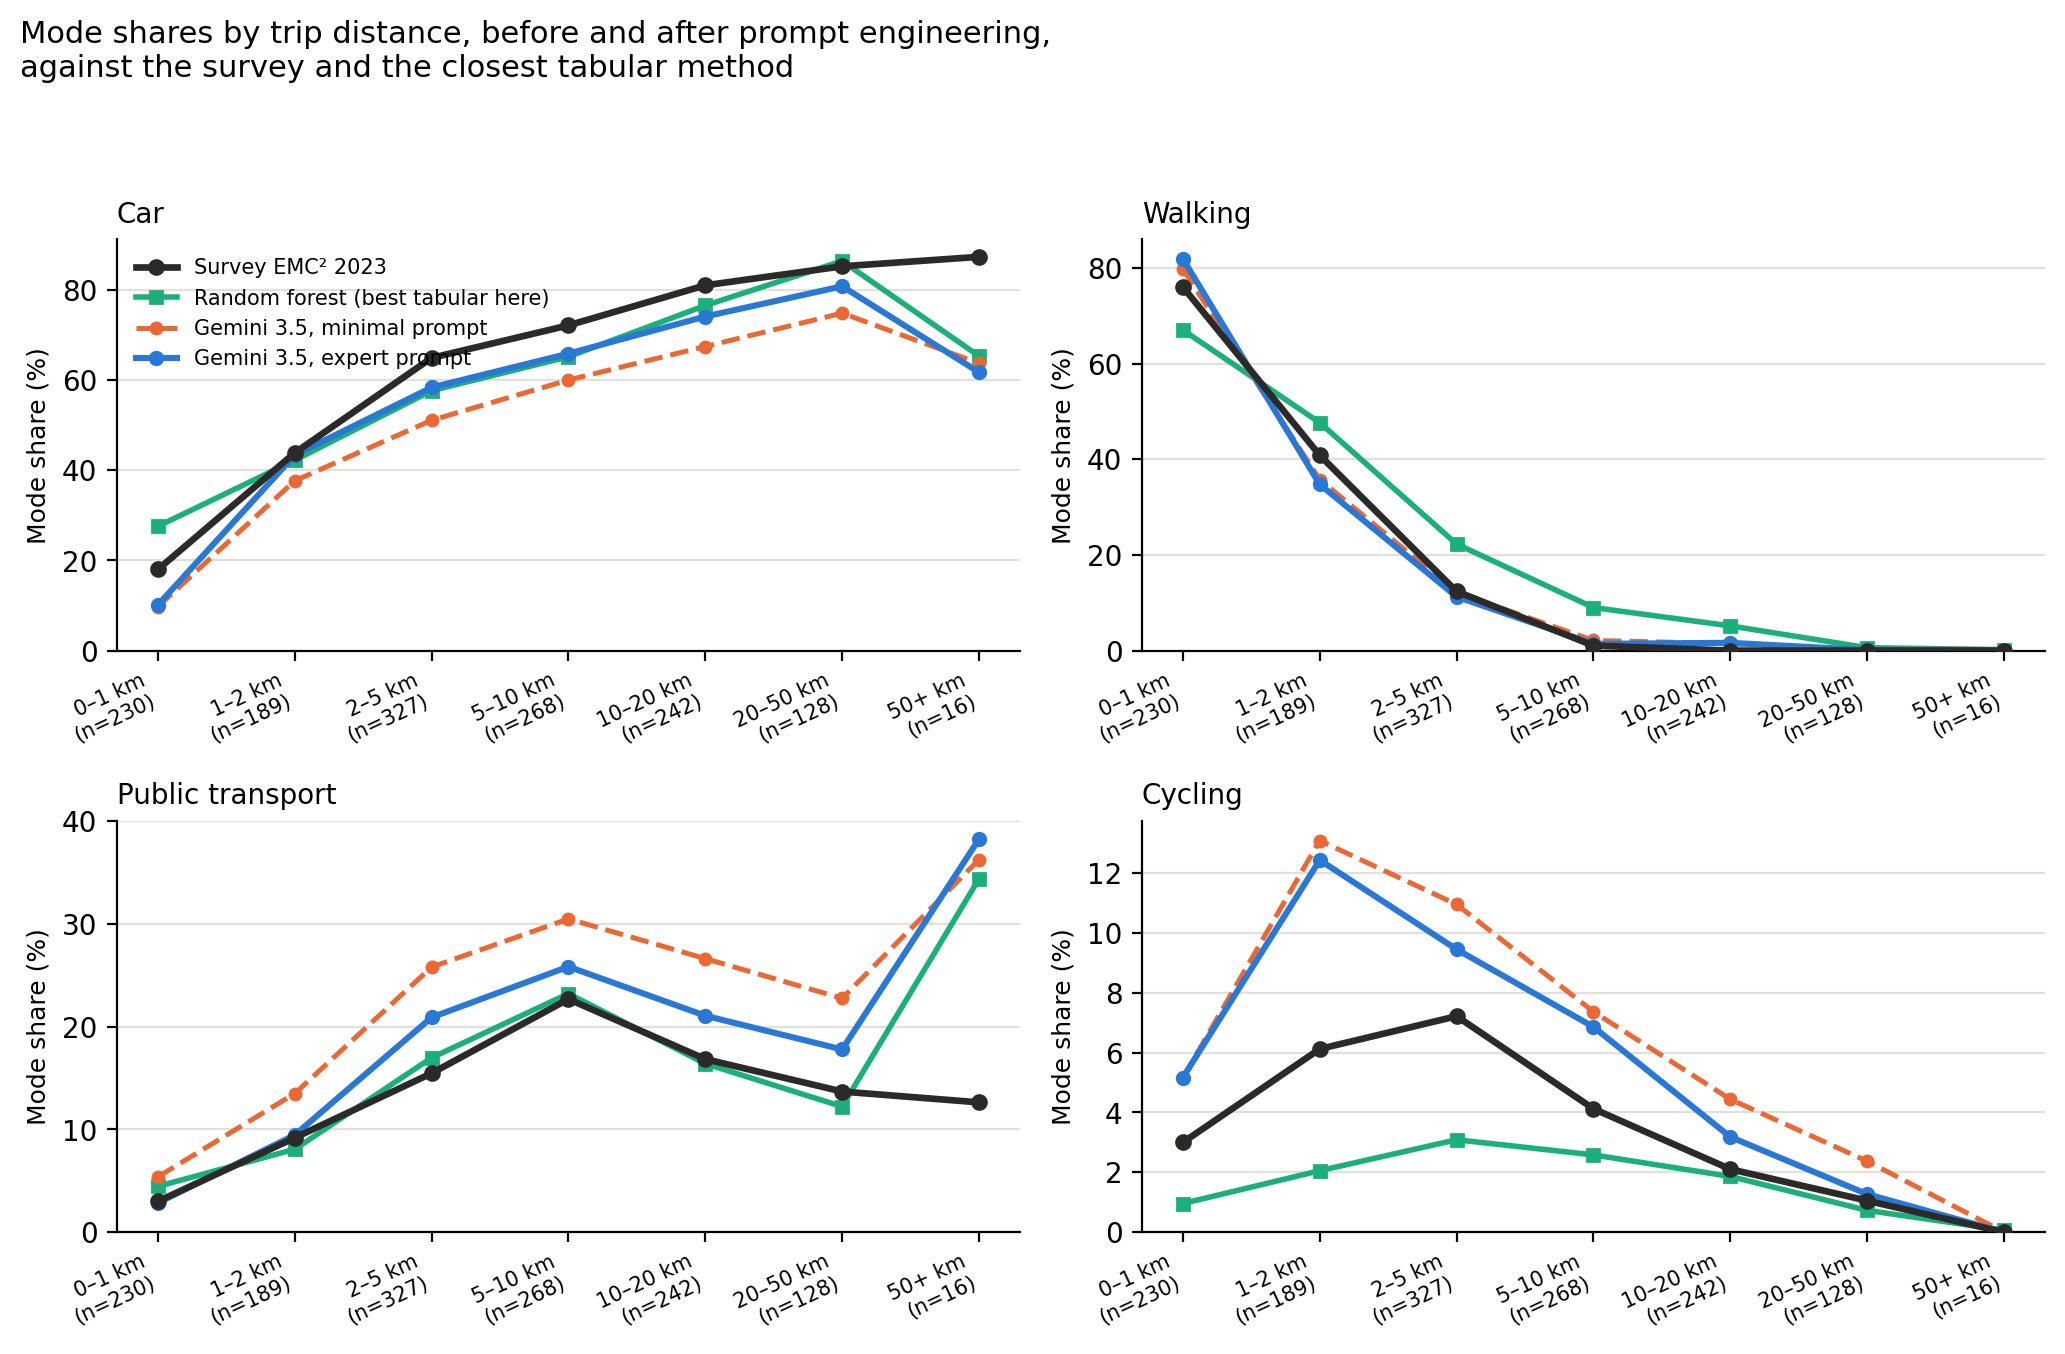
\includegraphics[width=\textwidth]{images/ch99_modes_distance.png}
  \caption{The four modes by distance band, one panel per mode. Car and walking land on the target from one kilometre onwards; public transport is overestimated by two to five points between two and twenty kilometres, and cycling by a factor of two on every band where it weighs. The tabular method errs the other way on cycling, which it places below the target everywhere.}
  \label{fig:app-modes-distance}
  \Description{Four panels, one per transport mode: car, walking, public transport and cycling. In each panel the horizontal axis carries the five distance bands and the vertical axis the modal share in per cent. Four curves are drawn: the survey target, the agent under the minimal prompt, the agent under the expert prompt, and a tabular reference. On the car and walking panels the expert-prompt curve meets the target curve from one kilometre onwards. On the public transport panel the agent curves stay two to five points above the target between two and twenty kilometres. On the cycling panel the agent curves sit at about twice the target on every band where cycling has weight, while the tabular curve sits below the target everywhere.}
\end{figure*}

\begin{figure*}[tp]
  \centering
  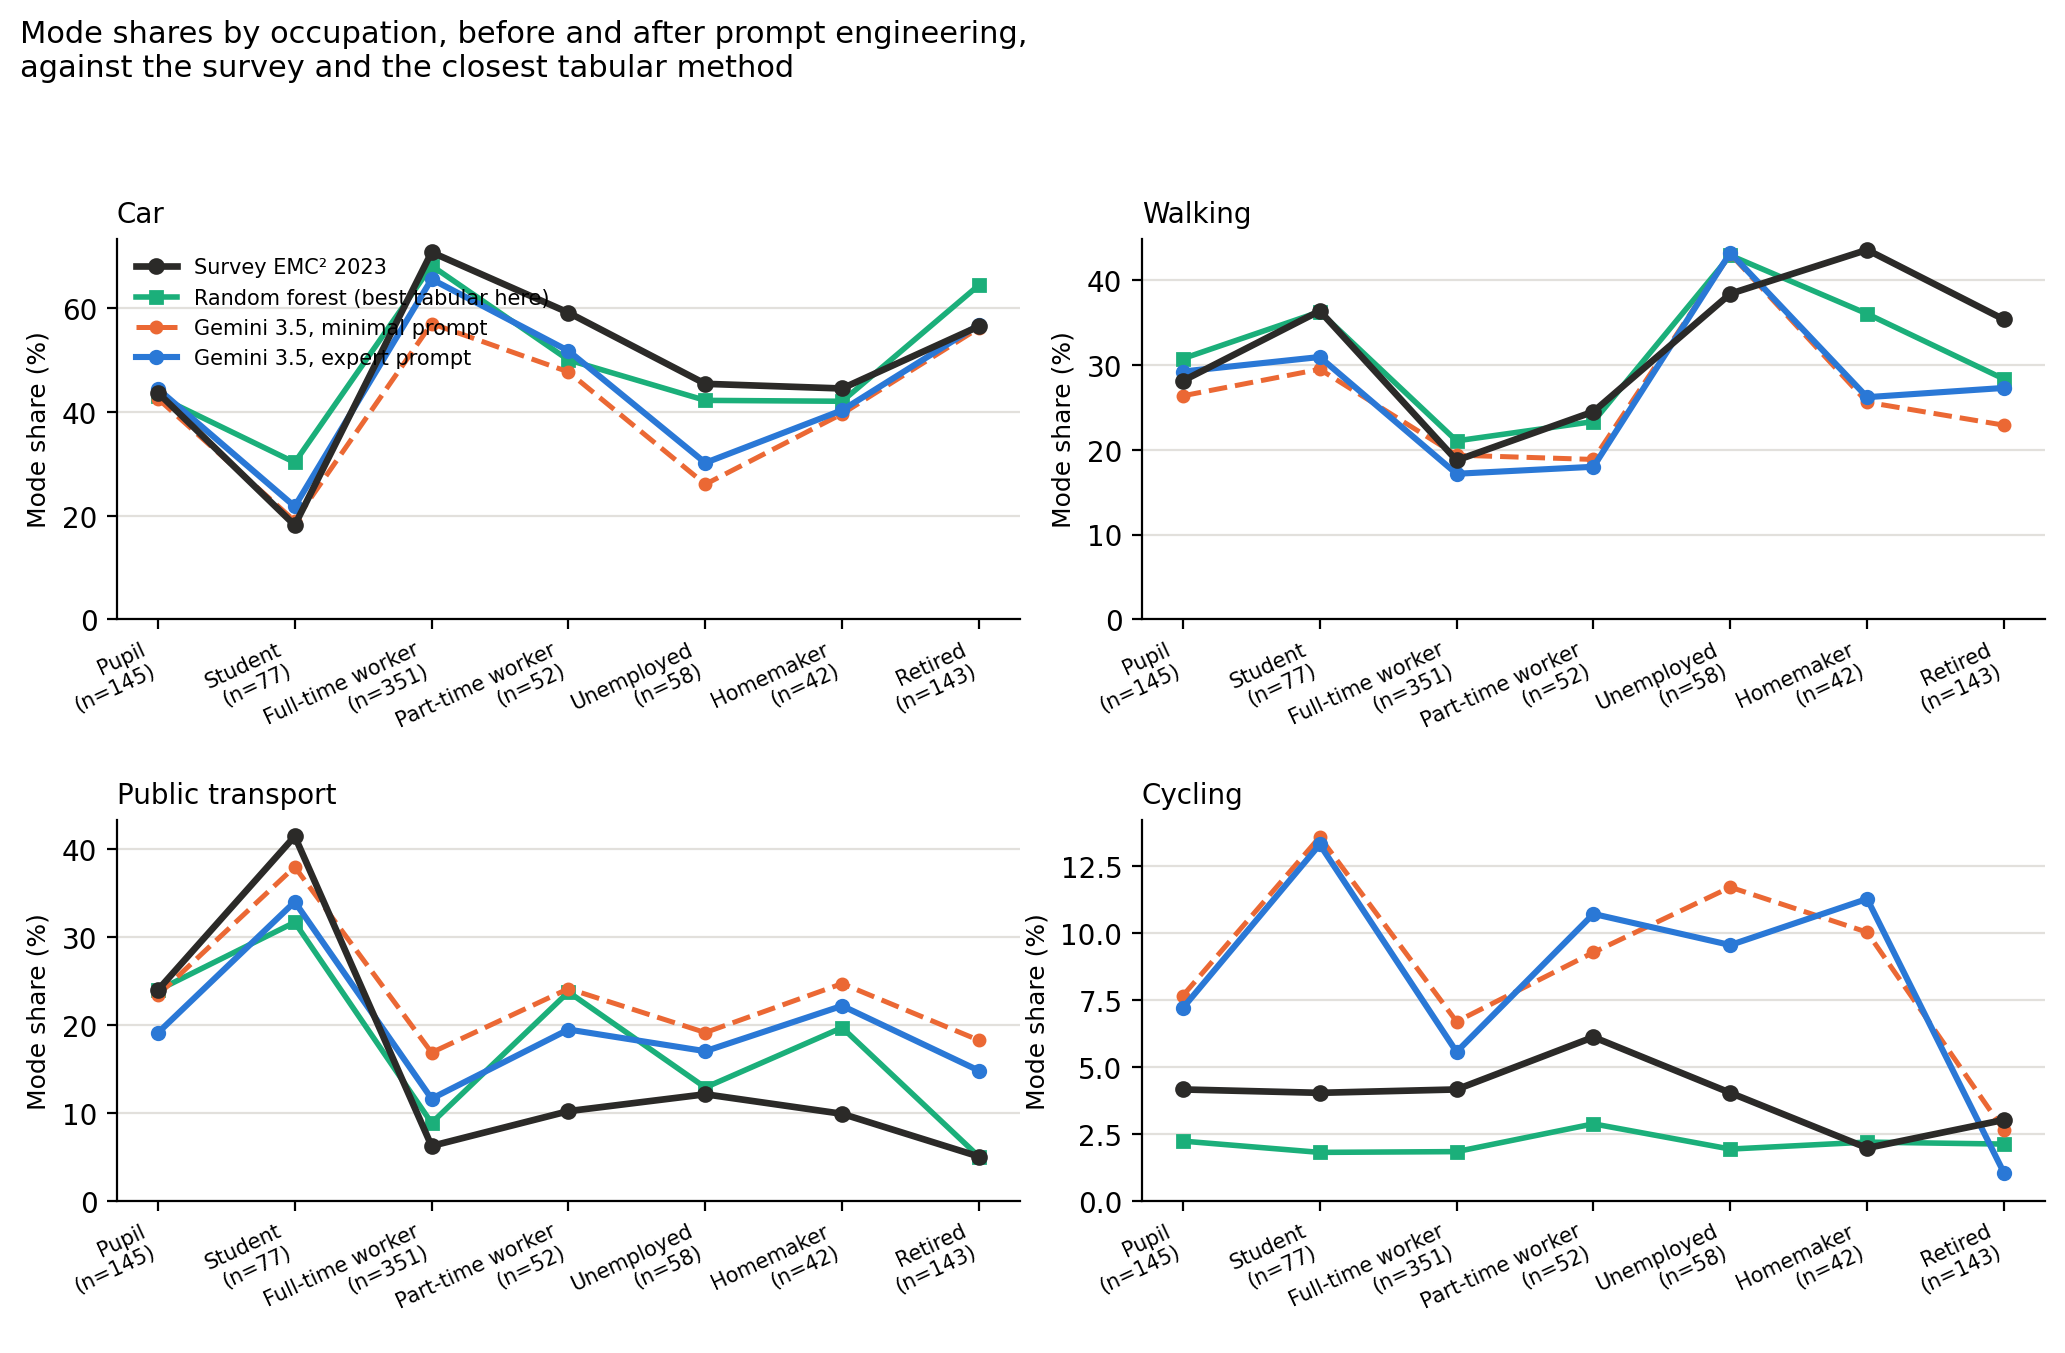
\includegraphics[width=\textwidth]{images/ch99_modes_occupation.png}
  \caption{The four modes read by occupation, same curves as Figure~\ref{fig:app-modes-distance}. The two school-age strata, pupils and students, are those where the agent places cycling highest: 8.2 and 13.3\,\% under the expert prompt, against 4.2 and 4.0\,\% in the survey. Student public transport goes from 37.9 to 35.5\,\% after tuning where the target is 41.4\,\%: tuning moves it away from the target on that stratum.}
  \label{fig:app-modes-occupation}
  \Description{Four panels, one per transport mode, with the eight occupation categories on the horizontal axis and the modal share in per cent on the vertical axis. The same four series are drawn as in the previous plate: survey target, agent under the minimal prompt, agent under the expert prompt, tabular reference. On the cycling panel the two school-age categories, pupils and students, carry the highest agent values of the plate, 8.2 and 13.3 per cent under the expert prompt against 4.2 and 4.0 per cent in the survey. On the public transport panel the student bar for the expert prompt sits lower than the bar for the minimal prompt, 35.5 against 37.9 per cent, while the target is 41.4, so the expert prompt moves away from the target on that stratum.}
\end{figure*}

\begin{figure*}[tp]
  \centering
  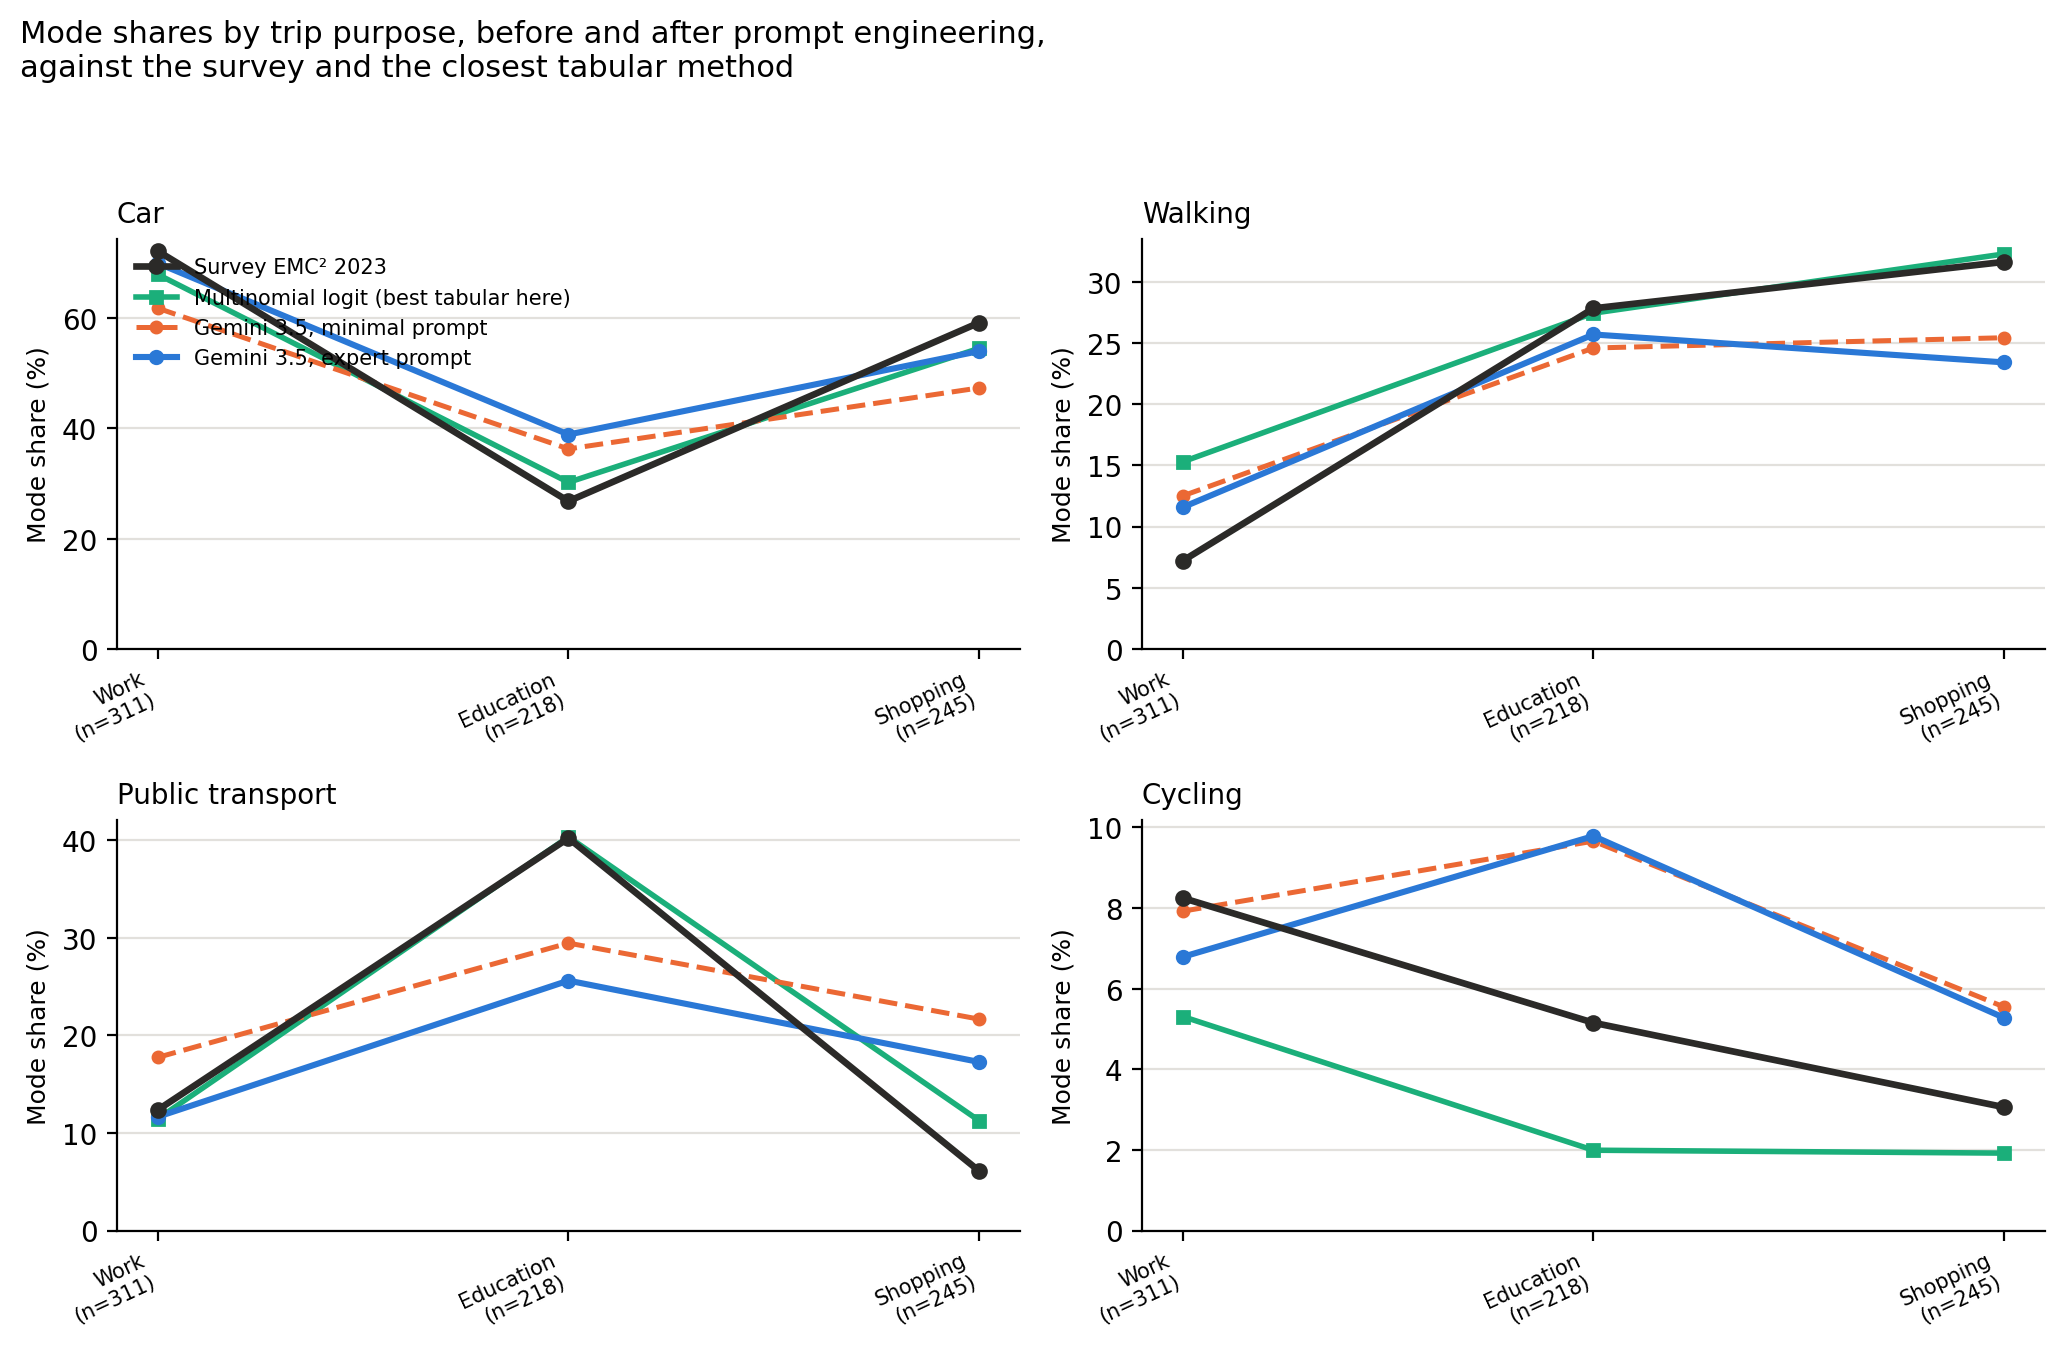
\includegraphics[width=\textwidth]{images/ch99_modes_motif.png}
  \caption{The four modes by trip purpose. Education is the purpose where the agent moves furthest from the target after tuning, and it moves away in the direction of the car, on a population that none of the four principles targets.}
  \label{fig:app-modes-motif}
  \Description{Four panels, one per transport mode, with the six trip purposes on the horizontal axis, home, work, education, shopping, leisure and other, and the modal share in per cent on the vertical axis. The same four series are drawn. On the car panel the education purpose shows the expert-prompt series above both the minimal-prompt series and the target, which is the largest such gap of the plate; the corresponding deficit appears on the public transport panel for the same purpose.}
\end{figure*}

\subsection{The modal shares of each decider}

\begin{table*}[tp]
  \caption{Global modal shares (\%) of every decider, against the survey. Every decider underestimates the car, an effect of the chain constraint that weighs on all of them in the chained reading. The two families err in opposite directions on cycling.}
  \label{tab:shares}
  \begin{tabular}{lrrrr}
    \toprule
    Decider & Car & Walking & Public transport & Cycling \\
    \midrule
    EMC\textsuperscript{2} 2023 survey     & 56.7 & 26.8 & 12.4 & 4.1 \\
    \midrule
    Minimal prompt, \texttt{gemini-3.5}    & 47.4 & 24.0 & 20.9 & 7.6 \\
    Expert prompt, \texttt{gemini-3.5}     & 52.3 & 24.2 & 16.6 & 6.8 \\
    Minimal prompt, \texttt{gemini-3.1}    & 44.1 & 19.5 & 28.8 & 7.7 \\
    Expert prompt, \texttt{gemini-3.1}     & 46.2 & 21.7 & 24.8 & 7.4 \\
    Minimal prompt, \texttt{mistral-large} & 36.7 & 24.4 & 30.6 & 8.2 \\
    Expert prompt, \texttt{mistral-large}  & 43.4 & 29.3 & 19.2 & 8.1 \\
    \midrule
    Gradient boosting                      & 52.8 & 29.1 & 14.8 & 3.3 \\
    Random forest                          & 56.2 & 27.6 & 14.2 & 2.0 \\
    Kernel logistic regression             & 54.4 & 28.9 & 13.6 & 3.0 \\
    Multinomial logit                      & 53.3 & 27.2 & 16.4 & 3.0 \\
    \bottomrule
  \end{tabular}
\end{table*}

\subsection{The strata that tuning degrades}

\begin{table}[tbp]
  \caption{Stratum L1 error (\%) before and after prompt engineering, on the two strata where tuning degrades the fit.}
  \label{tab:degraded}
  \small
  \setlength{\tabcolsep}{4pt}
  \begin{tabularx}{\columnwidth}{@{}Lrr@{}}
    \toprule
    Stratum and model & \multicolumn{1}{c}{Minimal} & \multicolumn{1}{c}{Expert} \\
    \midrule
    Education, \texttt{gemini-3.5} ($n = 218$)    & 28.0 & 33.5 \\
    Education, \texttt{gemini-3.1} ($n = 218$)    & 20.0 & 21.2 \\
    Education, \texttt{mistral-large} ($n = 218$) &  8.7 & 22.3 \\
    15--19 years, \texttt{gemini-3.5} ($n = 61$)    & 53.4 & 58.3 \\
    15--19 years, \texttt{gemini-3.1} ($n = 61$)    & 49.2 & 47.9 \\
    15--19 years, \texttt{mistral-large} ($n = 61$) & 34.1 & 44.9 \\
    \bottomrule
  \end{tabularx}
\end{table}

The degradation of the education purpose appears on all three models, that of the 15--19 year olds on \texttt{gemini-3.5} and \texttt{mistral-large}. Two strata otherwise resist every decider, tabular methods included: the 15--19 year olds, from 38 to 58 points of error, and trips over 50 kilometres, from 42 to 72 points over sixteen to nineteen decisions depending on the decider.

\subsection{Decision-by-decision agreement}

\begin{table*}[tp]
  \caption{Agreement between deciders over the trips carrying at least two options offered to both, 2{,}374 to 2{,}479 depending on the pair. The median gap between the distributions of two agents is four times the one that separates two tabular methods.}
  \label{tab:agreement-full}
  \small
  \setlength{\tabcolsep}{4pt}
  \begin{tabular}{@{}lrrr@{}}
    \toprule
    Pair & Most likely mode & Drawn mode & Median L1 between distributions \\
    \midrule
    Gradient boosting / kernel regression & 91.6\,\% & 90.5\,\% & 8.3 \\
    Gradient boosting / random forest     & 89.0\,\% & 88.3\,\% & 11.3 \\
    \midrule
    Expert \texttt{gemini-3.5} / gradient boosting & 69.7\,\% & 61.4\,\% & 39.0 \\
    Expert \texttt{gemini-3.5} / random forest     & 71.4\,\% & 60.4\,\% & 42.6 \\
    Expert \texttt{gemini-3.5} / expert \texttt{gemini-3.1}    & 79.6\,\% & 72.8\,\% & 40.0 \\
    Expert \texttt{gemini-3.1} / expert \texttt{mistral-large} & 72.6\,\% & 70.6\,\% & 40.0 \\
    \bottomrule
  \end{tabular}
\end{table*}

\subsection{The prompt variants and their scores}

\begin{table*}[tp]
  \caption{The prompt variants measured on \texttt{gemini-3.5-flash-lite}. The three expert variants saw the cohort, to different degrees: two were rewritten on its residuals, the third touched it only through the retention of one ablation. The first two were meant to give an upper bound; they do worse than the third.}
  \label{tab:variants}
  \small
  \setlength{\tabcolsep}{5pt}
  \begin{tabular}{@{}llrrr@{}}
    \toprule
    Variant & Status & Comp. & Excl.\ s.c. & L1 \\
    \midrule
    \texttt{prompt\_minimal\_02} & no engineering        & 7.02 & 10.39 & 24.08 \\
    \texttt{prompt\_expert\_05}  & ablation kept in view of the cohort & 4.86 &  6.86 & 13.85 \\
    \texttt{prompt\_expert\_06}  & tuned in sight of the cohort & 5.33 & 7.24 & 15.39 \\
    \texttt{prompt\_expert\_08}  & tuned in sight of the cohort & 6.58 & 10.32 & 21.74 \\
    \bottomrule
  \end{tabular}
\end{table*}

What the protocol foresaw as an in-sample fitting ceiling is not reached by the prompts that had access to it.

% =====================================================================
\section{The unit audit, decider by decider}
\label{app:unit}

The substrate differs from that of Appendix~\ref{app:detail}: the days the respondents actually described, 9{,}621 trips made by 2{,}930 people, each carrying the declared mode, by the protocol of Section~\ref{sec:audit}. These figures do not compare with those of Appendix~\ref{app:detail}, which bear on the synthetic cohort.

\subsection{Overall agreement}

\begin{table}[tbp]
  \caption{Unit agreement of the nine deciders on the declared trips. The two hard baselines receive no cross-entropy, which is infinite from the first error on.}
  \label{tab:unit-overall}
  \small
  \setlength{\tabcolsep}{4pt}
  \begin{tabularx}{\columnwidth}{@{}Lrrrr@{}}
    \toprule
    Decider & \multicolumn{1}{c}{Weighted} & \multicolumn{1}{c}{Arbitrated} & \multicolumn{1}{c}{Cross-} & \multicolumn{1}{c}{GMPCA} \\
            & \multicolumn{1}{c}{acc.} &    & \multicolumn{1}{c}{ent.} & \\
    \midrule
    Gradient boosting           & 71.5 & 67.4 & 0.419 & 0.657 \\
    Kernel logistic regression  & 70.6 & 66.2 & 0.438 & 0.646 \\
    Random forest               & 69.9 & 65.5 & 0.445 & 0.641 \\
    Multinomial logit           & 68.6 & 64.2 & 0.478 & 0.620 \\
    Shortest duration           & 68.1 & 65.3 & ---   & ---   \\
    Expert prompt               & 67.6 & 65.2 & $\mathbf{0.356}$ & $\mathbf{0.701}$ \\
    All-car                     & 66.7 & 61.7 & ---   & ---   \\
    Minimal prompt              & 64.8 & 61.6 & 0.460 & 0.631 \\
    Uniform random              & 23.5 & 21.5 & 1.260 & 0.284 \\
    \bottomrule
  \end{tabularx}
\end{table}

The ordering reverses from one column to the next: the expert prompt is sixth on accuracy and first on cross-entropy.

\subsection{Precision and recall per mode}

\begin{table*}[tp]
  \caption{Precision and recall per mode, in per cent, for the nine deciders. Declared counts: 431 bike, 5{,}971 car, 1{,}562 transit, 1{,}652 walking.}
  \label{tab:unit-modes}
  \begin{tabular}{lcccc}
    \toprule
    Decider & bike & car & transit & walking \\
    \midrule
    Gradient boosting          & 27.3 / 20.4 & 85.3 / 79.0 & 53.8 / 61.7 & 53.2 / 63.4 \\
    Kernel logistic regression & 25.2 / 19.3 & 85.2 / 78.1 & 52.6 / 60.4 & 51.1 / 62.7 \\
    Random forest              & 25.5 / 13.9 & 84.5 / 77.2 & 51.2 / 60.6 & 50.8 / 64.0 \\
    Multinomial logit          & 24.2 / 18.3 & 84.3 / 76.8 & 49.1 / 57.5 & 49.1 / 60.0 \\
    Shortest duration          & 16.9 / 25.8 & 74.4 / 92.3 & 53.5 / 39.7 & 81.3 / 19.2 \\
    Expert prompt              & 15.0 / 22.5 & 80.1 / 80.4 & 49.7 / 55.2 & 62.9 / 47.2 \\
    All-car                    & 16.1 / \phantom{0}2.3 & 72.6 / 95.8 & 42.3 / 25.3 & 35.9 / 16.2 \\
    Minimal prompt             & 14.7 / 24.1 & 81.2 / 75.1 & 42.8 / 60.0 & 61.2 / 44.2 \\
    \bottomrule
  \end{tabular}
\end{table*}

Both levels recall bikes better than any fitted method, 22.5 and 24.1~\% against 20.4 for gradient boosting, and pay for it in precision, 15.0 and 14.7~\% against 27.3. They lose walking, recall 47.2 and 44.2~\% against 63.4. Their precision on walking is nonetheless the best of the table, 62.9~\%: when they announce walking they are right, they do not announce it often enough.

\subsection{The confusion matrix of the expert prompt}

\begin{table}[tbp]
  \caption{The expert prompt, declared mode against predicted mode, in trips.}
  \label{tab:unit-confusion}
  \small
  \setlength{\tabcolsep}{4pt}
  \begin{tabularx}{\columnwidth}{@{}Lrrrr@{}}
    \toprule
    Declared $\backslash$ predicted & \multicolumn{1}{c}{bike} & \multicolumn{1}{c}{car} & \multicolumn{1}{c}{transit} & \multicolumn{1}{c}{walking} \\
    \midrule
    bike    &  97 &  227 &  62 &  45 \\
    car     & 345 & 4{,}799 & 540 & 283 \\
    transit &  88 &  481 & 862 & 132 \\
    walking & 116 &  488 & 269 & 779 \\
    \bottomrule
  \end{tabularx}
\end{table}

The audit carries a ceiling: 1{,}295 trips, 13.5~\%, have their declared mode absent from the options presented, removed by the vehicle chain or by the option cap. No decider could find it. The count runs from 1{,}226 to 1{,}428 depending on the decider.

The two figures of this audit are in Section~\ref{sec:individual}, Figures~\ref{fig:audit-modes} and~\ref{fig:audit-distance}.
